\documentclass{article}

\usepackage[a4paper,margin=1.15in,footskip=0.25in]{geometry}

\usepackage{hyperref}
\usepackage[utf8]{inputenc}
\usepackage[english]{babel}
\usepackage{textpos}
\usepackage{textcomp}
\usepackage{amsmath}
\usepackage{amssymb}
\usepackage{amsfonts}
\usepackage{graphicx}
\usepackage{epstopdf}
\usepackage{algorithmic}
\usepackage{verbatim}
\usepackage{textcomp}
\usepackage{varwidth}
\usepackage[linesnumbered,ruled]{algorithm2e}

% For displaying code
\usepackage{listings}

% Theorem
\newtheorem{theorem}{Theorem}

% lists
\usepackage{outlines}
\usepackage{enumitem}
\newenvironment{tight_enum}{
\begin{enumerate}[label=\alph*.]
\setlength{\itemsep}{0pt}
\setlength{\parskip}{0pt}
}{\end{enumerate}}

% \subsubsubsection{}
\setcounter{secnumdepth}{5}
\setcounter{tocdepth}{5}
\newcommand\simpleparagraph[1]{%
  \stepcounter{paragraph}\paragraph*{\theparagraph\quad{}#1}}

\usepackage{listings}
\usepackage{color}
\usepackage{xcolor}
\usepackage{mdframed}

\definecolor{dkgreen}{rgb}{0,0.6,0}
\definecolor{gray}{rgb}{0.5,0.5,0.5}
\definecolor{mauve}{rgb}{0.58,0,0.82}

% \usepackage{courier}
\lstset{%frame=tb,
language=C++,
aboveskip=3mm,
belowskip=3mm,
showstringspaces=false,
columns=flexible,
basicstyle={\small\ttfamily},
numbers=none,
numberstyle=\tiny\color{gray},
keywordstyle=\color{blue},
commentstyle=\color{dkgreen},
stringstyle=\color{mauve},
breaklines=true,
breakatwhitespace=true,
tabsize=3
}

%%%%%%%%% BEGIN DOCUMENT %%%%%%%%%
%%%%%%%%% BEGIN DOCUMENT %%%%%%%%%
%%%%%%%%% BEGIN DOCUMENT %%%%%%%%%

%% Used tt when referring to function

\begin{document}

\title{Parallel Orthogonal Recursive Bisection}
\author{Team Metropolis: \\
		Jamshid 'James' Farzidayeri, JJ Lay, and Graham West}
\date{COMS 7900, Capstone}

\maketitle

\begin{abstract}
In our first project, we implemented a parallel sorting algorithm which utilized a local gradient-type optimization search to equalize the amount of data across different compute nodes in order to achieve maximum efficiency. In this project, we applied this algorithm to the problem of parallel orthogonal recursive bisection (ORB), i.e., the construction of $k$-d trees. In order to do this, we had to heavily modify the sorting algorithm in several ways, including 1) turning it into a callable function, 2) letting the rank 0 head node perform work while still managing the tasks, 3) incorporating the use of different MPI communicators, and 4) altering the adaptive binning technique for better convergence.

In this paper, we will discuss how our $k$-d tree algorithm works, how we solved the various issues plaguing parallel sort (mentioned above), and how we tested and validated our work. We conclude with a discussion of the major difficulties in completing this project and how these difficulties could be minimized in the future.
\end{abstract}


\tableofcontents


%%%%%%%%%%%%%
%%% NEW SECTION %%%
%%%%%%%%%%%%%
\section{Introduction}

% farzi
The purpose of this project was to create a parallel searching program by expanding on a previous parallel sorting project. Given a set of predetermined and imported data, we were to develop an orthogonal recursive bisection ORB algorithm that would facilitate in organizing the data into a KD tree. The KD tree will include information such as, daughters, parents, spacial indexing, center, and size of node. Additionally, the process should maximize the use of MPI and having multiple computing nodes performing the work. Because we will be having multiple computing nodes with MPI and eventually carry the tree into single computing nodes, the process will required both serial and parallel tree building and searching operations. The goal is to have an extremely efficient method of searching through the data. Eventually a search using three radii and twenty million points from an existing file will be performed and that output will be saved to a file for later comparison.

% farzi
\subsection{Workflow}
One of the major issues we encountered during our last project was overwriting each other’s GitHub submissions. Our resolution was to create a master branch and three sub branches. Each person was assigned a sub branch that they could modify as they pleased. However, a modification in the master branch parallel approved folder required two or more party members consent. This vastly reduced the amount of issues encountered during push/pull request.

Another adjustment we made for our development process was to write our code together and in an accommodating space as opposed to assigning individual sections of code. We met on a regular basis, generally starting during our scheduled class period and extending through the lunch period. This allowed us to catch errors quickly, avoid merge conflicts and most significantly improved everyone's knowledge of how each component of the code works. 
When the project was assigned each team member prototypes a version of serial KD tree in their preferred language. After several meetings it was determined that Graham’s MatLab implementation would be used as the guide for the project. 

\subsection{Variables and conventions}
%%% NOTE %%%
%%% NOTE %%%
% 1) be consistent with the indices:
% 2) say head node (not master node)
% 3) say worker (not node) whenever possible
%%% NOTE %%%
%%% NOTE %%%
Note that we distinguish between \textbf{tree} nodes and \textbf{compute} nodes to avoid confusion.

\begin{mdframed}[backgroundcolor=blue!20]
	Counts:
	\setlength\itemsep{0.1pt}
	\setlength\parskip{0.1pt}
	\begin{itemize}
		\setlength\itemsep{0.1pt}
		\setlength\parskip{0.1pt}
		\item $N$: number of nodes
		\item $M$: max number of allowed time steps
		\item $L$: number of lines to read per file
		\item $L_w$: number of lines on the $w$th worker
		\item $D$: total number of lines/data points
	\end{itemize}
\end{mdframed}

\begin{mdframed}[backgroundcolor=blue!20]
	Indices:
	\setlength\itemsep{0.1pt}
	\setlength\parskip{0.1pt}
	\begin{itemize}
		\setlength\itemsep{0.1pt}
		\setlength\parskip{0.1pt}
		\item $m = 0, \cdots, M$: the time step of the bin adaptation scheme (likely less than $M$)
		\item $n = 0, \cdots, W$: spans the nodes
		\item $i = 0, \cdots, N$: spans the bin edges/indices
		\item $j = 0, \cdots, N-1$: spans the bin counts (this will occasionally subscript binI/E as well)
		\item $\ell_w = 0, \cdots, L_n-1$: spans the lines on the $n$-th node
		\item $k = 0, \cdots, 3$: the data column being sorted
	\end{itemize}
\end{mdframed}

\begin{mdframed}[backgroundcolor=blue!20]
	Variables:
	\setlength\itemsep{0.1pt}
	\setlength\parskip{0.1pt}
	\begin{itemize}
		\setlength\itemsep{0.1pt}
		\setlength\parskip{0.1pt}
		\item $\textrm{data}^n_{4\ell+k}$: data point on $\ell$th line and $k$th column on the $n$-th node
		\item ${E}^m_j$: bin edges (0 indexed) at time step $m$
		\item ${I}^{n,m}_j$: bin indices on node $n$
		\item ${C}^{n,m}_j$: bin counts on node $n$ at time step $m$
		\item ${C}^m_j$: total bin counts on head node (sum of node C's) at time step $m$
	\end{itemize}
\end{mdframed}


%%%%%%%%%
%
% Section: Implementation
%
%%%%%%%%%

\section{Implementation}
%
% JJ
%
\textcolor{red}{Here we discuss our implementation of the code}

\textcolor{red}{we used C++ with C MPI calls, mpirun, qsub/qlogin, valgrind}

\begin{center}

\includegraphics[width=0.95\textwidth]{images/flow.png}
\end{center}

%%%%%%%%%
%
% Subsection: Development
%
%%%%%%%%%

\subsection{Development}

The application was developed in a mixture of C and C++ on a Linux cluster. The compiler for the project was \texttt{g++} version 4.8.5-28 with the switch \texttt{-std=c++11} in order to utilize features introduced with that standard. The three most commonly used C++11 standards were placeholder type specifiers (i.e., \texttt{auto}), range based \texttt{for} loops, and the \texttt{nullptr} constant.

The C interface to MPI was selected for its familiarity and general support. While there are object-oriented C++ libraries such as \texttt{Boost.MPI} the authors elected to use the C version as they had experience with that environment and time to learn a new library was a limiting factor. Another concern was the installation of alternative libraries beyond Open MPI 2.1.1.

Debugging was performed using the tools \texttt{gdb} and \texttt{valgrind}. \texttt{gdb} was used primarily while developing the serial code for building the tree to identify the source of segmentation faults. \texttt{valgrind} was instrumental in locating memory leaks and illegal memory references during the parallel development. Code was executed with the command:

\begin{lstlisting}{language=bash}
mpirun -np 4 valgrind ./main > dump.txt 2> dump2.txt
\end{lstlisting}


One major challenge during the debugging process was that output was not displayed in chronological order making it difficult to understand the flow of the code. A solution we implemented was to print a numeric identifier during the execution at the beginning of each line. Each section of code was assigned a five digit numeric value, and the \texttt{mpi} rank was printed along with this. 

\begin{mdframed}[backgroundcolor=blue!20]
	\setlength\itemsep{0.1pt}
	\setlength\parskip{0.1pt}
	\begin{verbatim}
39300 : receiveFiles: Rank 93 received /home/hal2a/localstorage/public/
                              coms7900-data/datafile00122.txt as tag 0
39301 : receiveFiles: Rank 93 received DONE! as tag 1
35400 : receiveFiles: Rank 54 received /home/hal2a/localstorage/public/
                              coms7900-data/datafile00157.txt as tag 0
35401 : receiveFiles: Rank 54 received /home/hal2a/localstorage/public/
                              coms7900-data/datafile00023.txt as tag 1
35402 : receiveFiles: Rank 54 received DONE! as tag 2
30000 : receiveFiles: Rank 0 received /home/hal2a/localstorage/public/
                              coms7900-data/datafile00407.txt as tag 0
39901 : receiveFiles: Rank 99 received DONE! as tag 1
30001 : receiveFiles: Rank 0 received /home/hal2a/localstorage/public/
                             coms7900-data/datafile00361.txt as tag 1
30002 : receiveFiles: Rank 0 received DONE! as tag 2
30900 : receiveFiles: Rank 9 received /home/hal2a/localstorage/public/
                             coms7900-data/datafile00020.txt as tag 0
30901 : receiveFiles: Rank 9 received /home/hal2a/localstorage/public/
                             coms7900-data/datafile00046.txt as tag 1
30902 : receiveFiles: Rank 9 received DONE! as tag 2
45700 : receiveFiles: Rank 157 received /home/hal2a/localstorage/public/
                               coms7900-data/datafile00086.txt as tag 0
45701 : receiveFiles: Rank 157 received DONE! as tag 1
70000 : Rank 11 is calling buildTree
70000 : Rank 70000 : Rank 125 is calling buildTree
70000 : Rank 131 is calling buildTree	
    \end{verbatim}
\end{mdframed}

The output was then sorted using:

\begin{lstlisting}{language=bash}
cat dump.txt | sort | less
\end{lstlisting}


Code was executed using both interactively by logging into a compute node using \texttt{qlogin} and as a batch job using \texttt{qsub}. Short runs of a few minutes were performed interactively when failures occurred quickly or to test a new section of code on smaller data sets. Longer runs that needed more than eight nodes were submitted to the Sun Grid Engine batch system.  

%%%%%%%%%
%
% Subsection: main
%
%%%%%%%%%

\subsection{\texttt{main}}
Our \texttt{main} program is divided into three main phases (each of which is comprised of multiple functions): data import, tree building, and tree searching. The data import phase collects all of the relevant filenames of the data files, reads them, and places them into a single 1D array. The tree building phase begins by initializing an empty Tree struct (see below for explanation of the struct) which is then passed into the \texttt{buildTree} function which alters the struct's contents. The entire tree can then be navigated by using the tree's left, right, and parent fields. The final tree searching phase takes the completed tree struct as an argument along with a search sphere. The number of points within the search sphere is calculated for each

There are four variables which govern the performance of the KD tree and the size of the problem. First are the number of data files to read and the number of lines to read per file. These values are set in the beginning of \texttt{main} and they have a maximum value of 500 and 20,000,000, respectively. Third, is the number of compute nodes. In general, increasing this number should speed up execution of the program. Its value is set in the command line when running the program and its value must be smaller than the number of files. Last, is the number of lines to read from the 501-st data file. These are the centers of the search spheres. The value is set in \texttt{search501}.


% import: gets the list of files and imports their data into an array

% build: we build the tree using ORB to partition the data

% search: import the 501-st data file and perform a search on each, summing the total number of points found over several radii


%%%%%%%%%
%
% Subsection: K-d Tree
%
%%%%%%%%%

\subsection{K-d tree}
%
% JJ, talk about the Tree struct and what all fields it has
%

The design of the k-d tree required storing information for organizing the parallel distribution of the data and the data held locally on the node. Rather than create two different type of structures, the code utilized a single C \texttt{struct} which originally was defined as:

\lstset{language=C++, keepspaces=true}
\begin{lstlisting}
struct Tree {
    // Pointers used for local tree
	Tree *p;    // Parent
	Tree *l;    // Left child
	Tree *r;    // Right child
	int i;      // Sort dimension used to split this node
	int source; // Which buildTree function created it

    // Pointers used for parallel tree
	MPI_Comm parentComm;  // Parent communicator
	MPI_Comm leftComm;    // Left child communicator
	MPI_Comm rightComm;   // Right child communicator
	MPI_Comm thisComm;    // Communicator that the node belongs to

    // Each node in the tree has a unique identifier
	string name;

    // For nodes with children, this holds the min and max for
    // the child nodes
	double x1;  // Min x
	double x2;  // Max x
	double y1;  // Min y
	double y2;  // Max y
	double z1;  // Min z
	double z2;  // Max z

	int depth;  // Depth of the node in the tree
	int n;      // Number of points

	double c[4];    // Center of this tree
	double radius;  // Radius of this tree

	double d[4];   // Data point coordinates
	double index;  // File row index from source data
}
\end{lstlisting}

Unfortunately, this structure proved to be too bloated when attempting to import all 10 billion rows of data as well as the 20 million rows of search rows. The simplified tree structure is:

\lstset{language=C++, keepspaces=true}
\begin{lstlisting}
struct Tree {
	Tree *p;  // Parent
	Tree *l;  // Left child
	Tree *r;  // Right child

	MPI_Comm parentComm, leftComm, rightComm, thisComm;

	float x1;  // Min x
	float x2;  // Max x
	float y1;  // Min y
	float y2;  // Max y
	float z1;  // Min z
	float z2;  // Max z

	float c[4];  // Center of this tree
	float radius;

	float d[4];  // Data point
}
\end{lstlisting}

Another change was moving from \texttt{double} data types to \texttt{float} in order to conserve memory.

During the parallel construction phase, nodes are separated into different MPI communicators as shown in Figure~\ref{fig:communicators}. The four \texttt{MPI\_Comm} variables store the references to the parent, child, and current communicators. The value \texttt{MPI\_COMM\_SELF} is used as a ``null'' value for these pointers to indicate no communicators exist in the given direction.

Once the nodes became members of a communicator containing only itself, \texttt{buildTree} constructed the local serial tree using the same structure but using the \texttt{Tree} pointers rather than the \texttt{MPI\_Comm} variables.


%%%%%%%%%
%
% Subsubsection: Constants
%
%%%%%%%%%

\subsubsection{Constants}\label{sec:constants}

C preprocessor identifiers were defined and used in place of numeric constants for readability. Data points were defined as an array of \texttt{double} of size four consistently even when only three values were needed. The four positions were referenced using:

\lstset{language=C++, keepspaces=true}
\begin{lstlisting}
#define _INDEX_   0  // Row index from source datafile
#define _X_       1
#define _Y_       2
#define _Z_       3
\end{lstlisting}

A single tree is create and populated by both the parallel and serial versions of \texttt{buildTree}. To aid with debugging, each node is marked with an identifier to show which function created it. The identifiers for the sources are:

\lstset{language=C++, keepspaces=true}
\begin{lstlisting}
#define _Source_buildTree_unknown     0
#define _Source_buildTree_parallel   -1
#define _Source_buildTree_serial     -2
\end{lstlisting}

%%%%%%%%%
%
% Subsubsection: Naming
%
%%%%%%%%%

\subsubsection{Tree Node Naming}

Each node in the tree is assigned a unique identifier determined by its position. The top node is named \texttt{t}. The two child nodes of \texttt{t} are \texttt{tl} and \texttt{tr}. An \texttt{l} or \texttt{r} is appended to the parent's name to designate the direction it is below the parent. The final node of the parallel section appends an \texttt{*} to designate the transition from parallel to serial. The node of the tree containing the data point appends an \texttt{!}.


%%%%%%%%%
%
% Subsubsection: Parallel Variable
%
%%%%%%%%%

\subsubsection{Parallel variables}

The \texttt{struct} variables used during the initial division of the tree among the nodes and their purpose are:

\begin{tabular}{l l}
\texttt{i} & The dimension that was split by the MPI communicator.  \\
\texttt{source} & During the parallel phase, this value is set to  \\
& \texttt{\_Source\_buildTree\_parallel}.  \\
\texttt{parentComm} & The parent MPI communicator that created this node. The\\
&  root node stores a value of \texttt{MPI\_COMM\_SELF} in lieu of a null. \\
\texttt{leftComm} & The MPI communicator of the \textit{left} child tree for the current node.  \\
\texttt{rightComm} & The MPI communicator of the \textit{right} child tree for the current node.  \\
\texttt{thisComm} & The MPI communicator of the current compute node.  \\
\texttt{name} & The unique name of the tree node. \\
\texttt{x1} & The minimum value of \textit{x} stored in this subtree.  \\
\texttt{x2} & The maximum value of \textit{x} stored in this subtree.  \\
\texttt{y1} & The minimum value of \textit{y} stored in this subtree.  \\
\texttt{y2} & The maximum value of \textit{y} stored in this subtree.  \\
\texttt{z1} & The minimum value of \textit{z} stored in this subtree.  \\
\texttt{z2} & The maximum value of \textit{z} stored in this subtree.  \\
\texttt{depth} & The depth within the tree of the current node. The top node has a \\
& depth of zero.  \\
\texttt{n} & The number of points contained within the subtree where the current \\
& node is the root.  \\
\texttt{c[4]} & The center of the subtree. Index for the array is described in section \ref{sec:constants}. \\
\texttt{radius} & The distance from the center of the subtree to the furthest point.  \\
\end{tabular}

\begin{center}
   \begin{figure}[h!]
      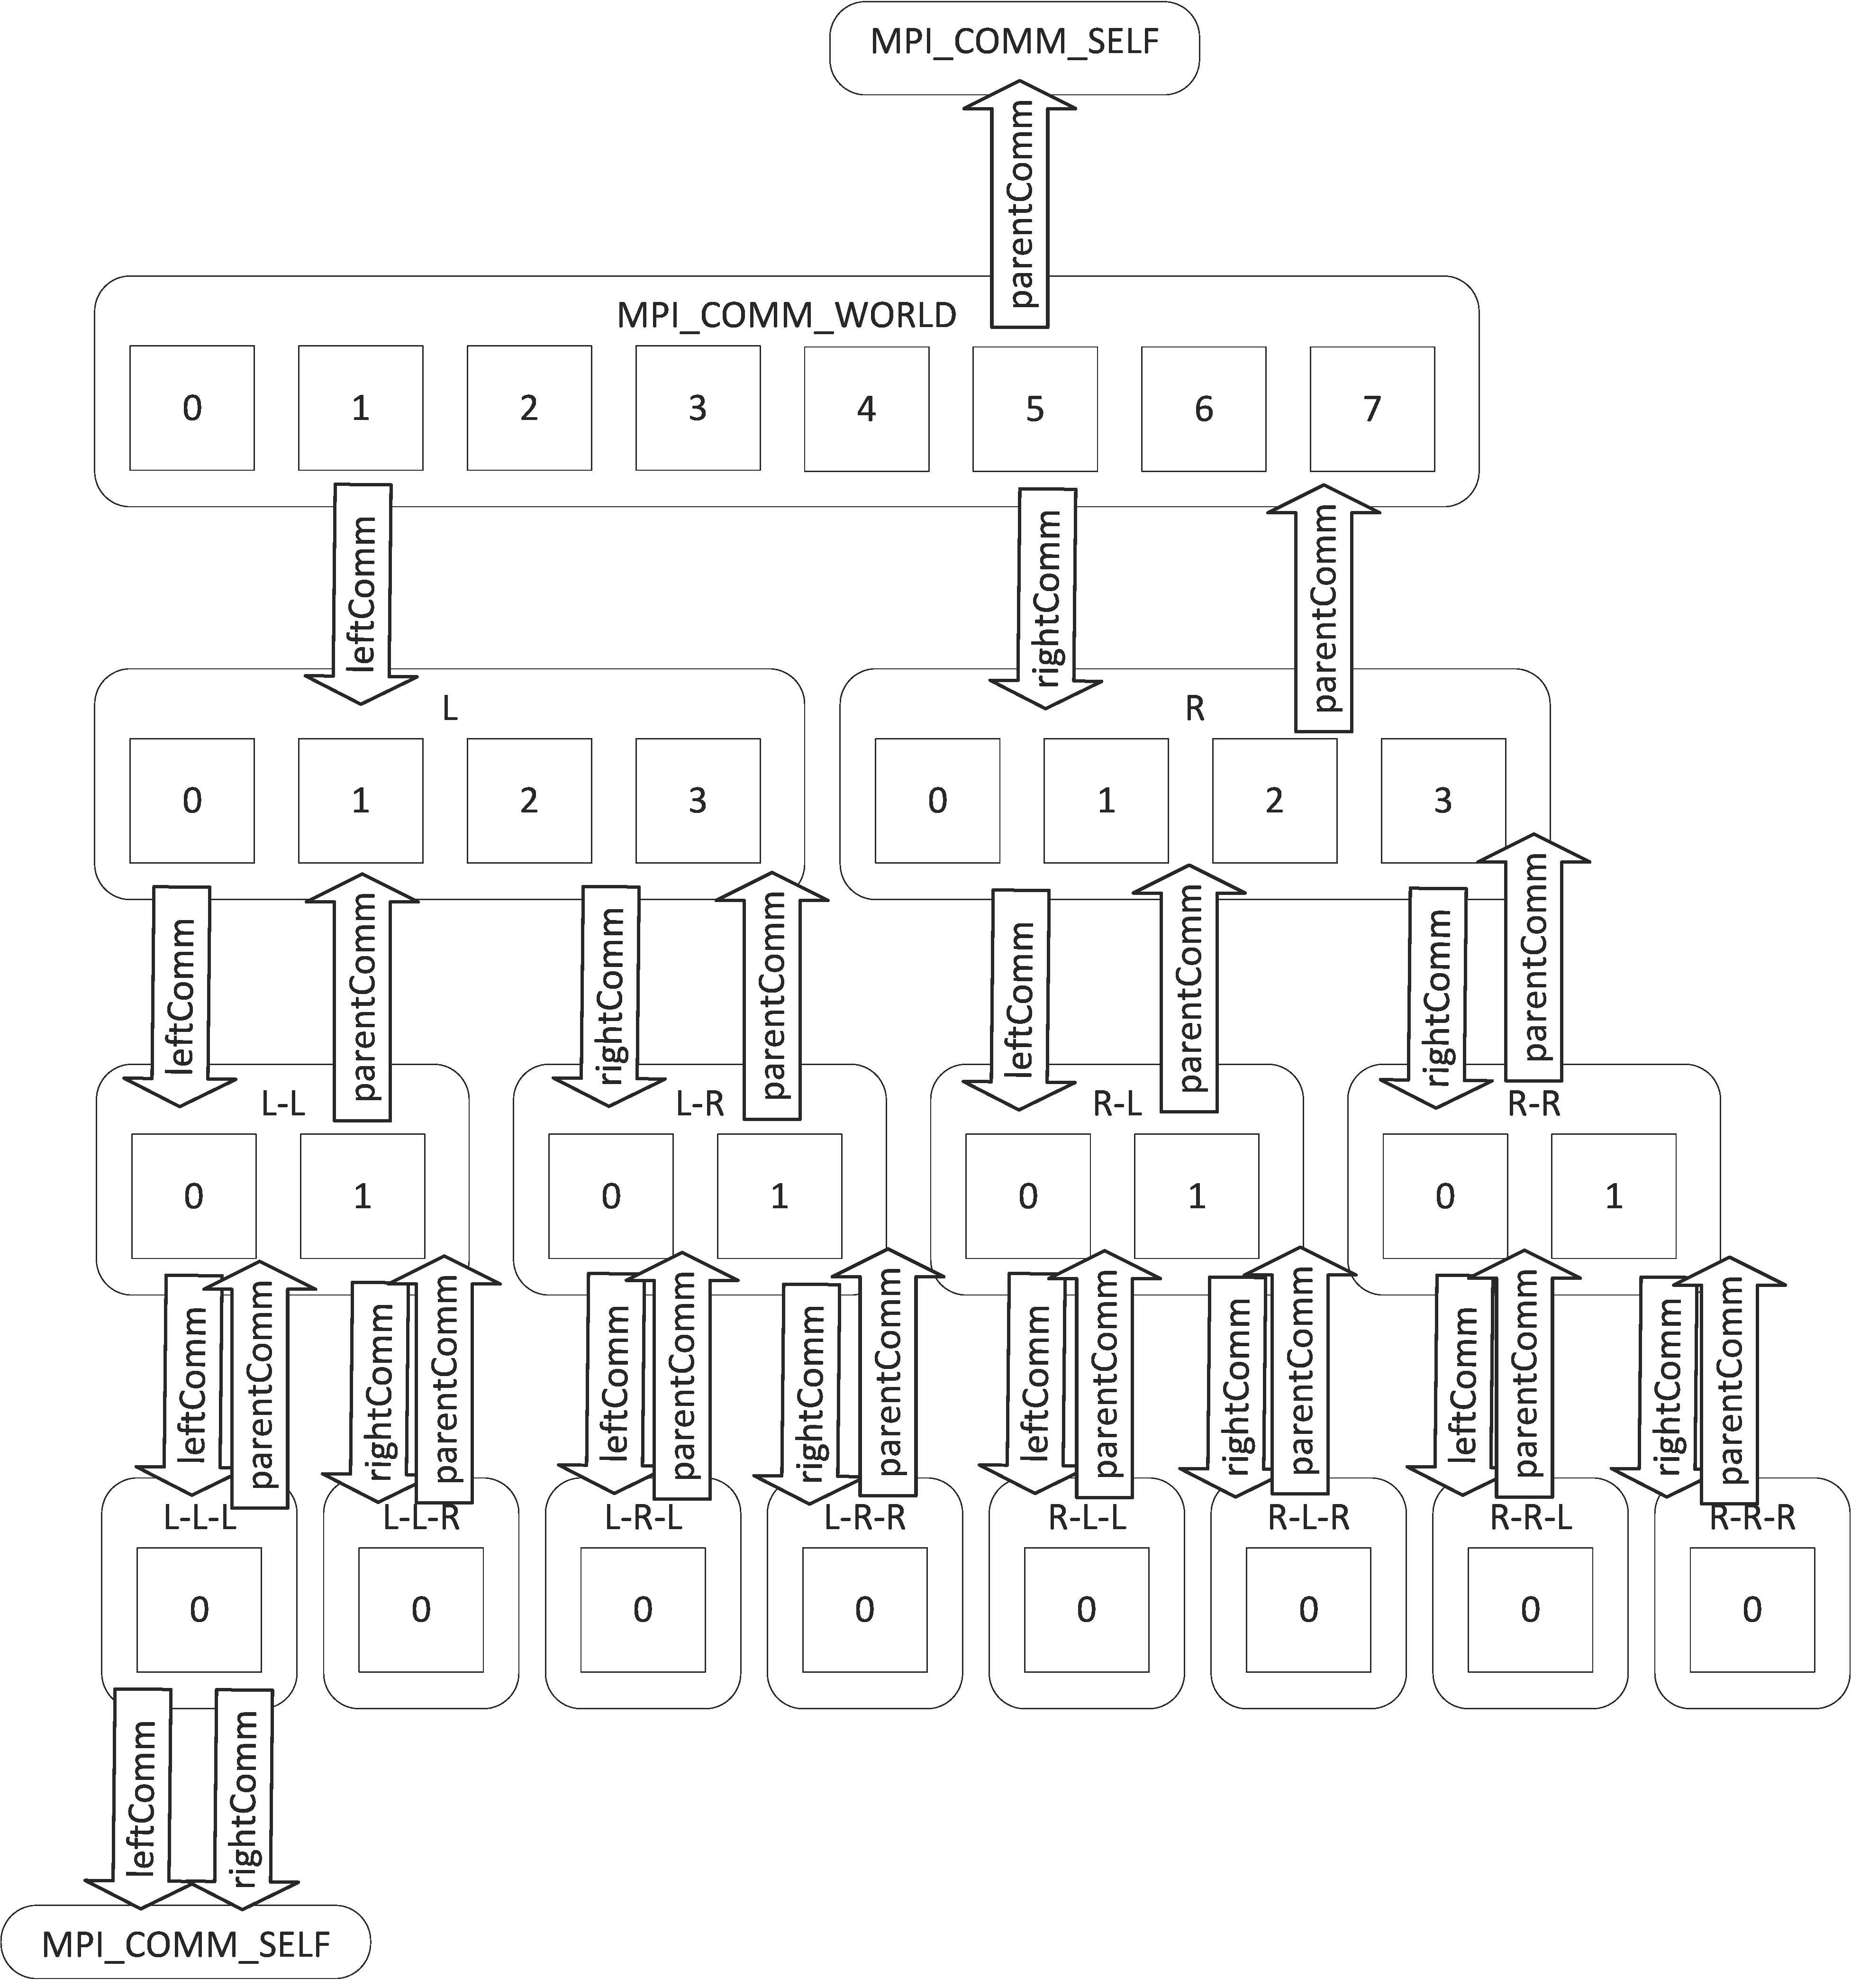
\includegraphics[width=0.9\textwidth]{images/communicators.png}
      \caption{Example of parallel variables using eight nodes}
      \label{fig:communicators}
   \end{figure}
\end{center}

%%%%%%%%%
%
% Subsubsection: Serial variables
%
%%%%%%%%%

\subsubsection{Serial variables}

The \texttt{struct} variables used during the final division of the local serial tree on the compute nodes and their purpose are:

\begin{tabular}{l l}
\texttt{p} & Pointer to the parent of the current node. This value is \texttt{null} for the top node. \\
\texttt{l} & Pointer to the \textit{left} child of the current node. This value is \texttt{null} for the data point. \\
\texttt{r} & Pointer to the \textit{right} child of the current node. This value is \texttt{null} for the data point. \\
\texttt{i} & The dimension that was split during the local tree construction. \\
\texttt{source} & During the serial phase, this value is set to \texttt{\_Source\_buildTree\_serial}. \\
\texttt{name} & The unique name of the node. \\
\texttt{x1} & The minimum value of \textit{x} stored in this subtree. \\
\texttt{x2} & The maximum value of \textit{x} stored in this subtree. \\
\texttt{y1} & The minimum value of \textit{y} stored in this subtree. \\
\texttt{y2} & The maximum value of \textit{y} stored in this subtree. \\
\texttt{z1} & The minimum value of \textit{z} stored in this subtree. \\
\texttt{z2} & The maximum value of \textit{z} stored in this subtree. \\
\texttt{depth} & The depth within the tree of the current node. The top node has a depth of zero. \\
\texttt{n} & The number of points contained within the subtree where the current node \\
& is the root. \\
\texttt{c[4]} & The center of the subtree. Index for the array is described in section \ref{sec:constants}. \\
\texttt{radius} & The distance from the center of the subtree to the furthest point. \\
\end{tabular}


%%%%%%%%%
%
% Subsubsection: Data point variables
%
%%%%%%%%%

\subsubsection{Data point variables}

The \texttt{struct} variables used for storing the data point within the tree and their purpose are:

\begin{tabular}{l l}
 \texttt{p} & Pointer to the parent of the current node.  \\
 \texttt{l} & Pointer to the \textit{left} child of the current node. This value is \texttt{null} for the data point.  \\
 \texttt{r} & Pointer to the \textit{right} child of the current node. This value is \texttt{null} for the data point.  \\
 \texttt{source} & During the serial phase, this value is set to \texttt{\_Source\_buildTree\_serial}.  \\
 \texttt{name} & The unique name of the node.  \\
 \texttt{depth} & The depth within the tree of the current node. The top node has a depth of zero.  \\
 \texttt{n} & The number of points contained within the subtree where the current node is the root.  \\
 \texttt{d[4]} & The data point.  \\
 \texttt{index} & The row index of the data point as read from the source file.  \\
 \end{tabular}


%%%%%%%%%
%
% Subsection: Building the tree
%
%%%%%%%%%

\subsubsection{Building the tree}
% General notes on the method...

\paragraph{\texttt{buildTree}}
% farzi, just add the listing
This function gets the number of compute nodes $q$ available in the current communicator and determines which function to run. If $q>1$, then we can still do a parallel sort with at least two compute nodes, so \texttt{buildTree\_parallel} is entered. If $q=1$, then \texttt{buildTree\_serial} is entered.


%%%%%%%%%
%
% Function: buildTree_serial
%
%%%%%%%%%

\paragraph{\texttt{buildTree\_serial}}
This was the first function written after our initial prototyping phase was completed. It essentially performs a serial version of ORB which can be executed on a single compute node.

%
% JJ, you wanna write this since you wrote the program?
%

Upon completion, \texttt{buildTree\_serial} recursively calls itself instead of \texttt{buildTree} since we still have $q=1$.


\paragraph{\texttt{buildTree\_parallel}}
This function performs essentially the same tasks as \texttt{buildTree\_serial}, but utilizing multiple nodes for speedup. Specifically, it takes advantage of \texttt{parallelSort} in order to speed up the partitioning of the data along the longest axis (determine by \texttt{getSortDim}, discussed below). After the data has been sorted, the data is split by placing lower half (w.r.t. the sorted data values) of the compute nodes into a left communicator and the upper half into a right communicator. Each half then calls \texttt{buildTree}.

% Upon completion, \texttt{buildTree\_parallel} has spawned 2 new communicators (a left and a right) each of which has half as many compute nodes as the parent communicator. All of the nodes from each side then call \texttt{buildTree} so that they can perform the $q$ check.


\paragraph{\texttt{getSortDim}}
This function is used by \texttt{buildTree\_parallel} in order to determine which is the longest axis, i.e., the sort dimension. In addition to this, it also fills in the struct for the current tree node with the global min/max in all three dimensions. To do this, each node gets its own min/max for each axis and sends them to rank 0 (w.r.t. the current communicator). Rank 0 then determines the global min/max and them MPI\_Bcast's those values back to the other ranks. This allows each communicator to sort their data independently along different axes. The center of the bounding box defined by these values min's/max's is also stored in the tree struct. 


\subsubsection{Searching the tree}



\paragraph{\texttt{searchTree\_serial}}
% GW
This function is called by all ranks and returns an integer which equals the number of points found by the rank that called it. It takes as arguments the point and radius (which specifies a search sphere) and the root of the tree created by \texttt{buildTree}. To perform the search, a check is done to determine of the search sphere intersects the bounding sphere of each data partition:
\begin{equation}
		r^2_\textrm{sphere center to box center} \le (r_{sphere} + r_{box})^2
\end{equation}
We used the squared version of the formula to avoid computing the square root, thus saving time. If this check returns false, then there are no data points within the search sphere contained in that partition and the function exits. If true, then another check is performed to check if the left or right child tree are NULL. If they are both NULL, then by our definition of the tree, we have found a point that is a leaf of the tree, thus we increment the count and exit the function. Otherwise, we recursively call the function again using the correct child tree.

%%%%%%%%%
%
% Function: search501
%
%%%%%%%%%

\paragraph{\texttt{search501}}
%
% JJ, edit if you wan since you wrote most of this
%

Each compute node calls this function which reads the data file \texttt{datafile00501.txt} whose contents are the centers of the search spheres. It then loops \texttt{searchTree\_serial} for all of the sphere centers for three different radii (0.01, 0.05, 0.10). The counts on each compute node are then stored. After all searches are complete, an \texttt{MPI\_Reduce} is performed by all nodes, thus adding all of the counts into a single array which is sent to \texttt{stdout}. When the job is submitted using \texttt{qsub}, the output is directed to a file with the name of the job.


\subsection{Altered parallel sorting}
We had to adjust our parallel sorting algorithm a great extend to integrate it into the new project.


\subsubsection{\texttt{parallelSort}}

% GW, farzi

\paragraph{Conversion to function}
One of our first obstacles was modifying our original \texttt{parallelSort}  program to work for this project. The first issue was having \texttt{parallelSort} operate as a function. We accomplished this by removing the MPI setup and Data Import sections from \texttt{parallelSort} and placing them into a new Main. While doing this we encountered issues with how the data was passed using both a pointer and array notation. Because several functions within the \texttt{parallelSort} function would need to change both the number of rows and the data we had to pass as pointers and pointers to arrays. 


\paragraph{Making rank 0 do work}
The second issue was our use of rank 0 which as the manager in our original \texttt{parallelSort} program. Our implantation of \texttt{parallelSort} had rank 0 manage while all the other ranks were compute nodes which contained and performed operations on the actual data. However, when utilizing a KD tree all of the ranks are needed as compute nodes otherwise each time the tree forked and a new communication branch was formed the process would lose a rank due to a new rank 0 being formed. To resolve this problem we had to make several clever adjustments in the sections of the code, most notably the adapt binning section. Other sections just needed to have the iteration increment from 0 instead of 1.

\paragraph{Using different communicators}
Since kdtree requires multiple comms, it was necessary that \texttt{parallelSort} (any many functions it contains) was given the current communicator. This was not a terribly difficult modification, but it was quite tedious since there were many functions which required alterations to their header files.


\subsubsection{\texttt{adaptBins}}
Although our original adaptive binning scheme performed well, we wanted something which could do even better since $k$-d trees require many parallelSort calls. As a review, here is our original method:
\begin{equation}
	\begin{split}
		\Delta C & = 2.0 ( C^{m}_{i+1} - C^{m}_i ) / ( C^{m}_{i+1} + C^{m}_i ) \\
		\Delta E & = E^m_{i+1} - E^m_i \\
		E^{m+1}_i & = E^m_i + \alpha \Delta C \Delta E
	\end{split}
\end{equation}
% added scale factor
where $C$ are the bin counts, $E$ are the bin edges, and $\alpha < 0.5$. This method will occasionally devolve into oscillatory behavior and not converge to the correct value. To combat this in the $k$-d tree project, we added a scale factor $S$ which decreases over time:
\begin{equation}
	\begin{split}
		S(m) & = 1 - (1 - 0.1) (1 - \textrm{exp}(-0.03 m) \\
		E^{m+1}_i & = E^m_i + \alpha S(m) \Delta C \Delta E
	\end{split}
\end{equation}

Since this method is local, it converges slowly at bin edges far away from high-density clusters. As such, we attempted to replace this method with a global method which uses linear interpolation to estimate where the bins would be evenly distributed. Define the function $\hat C(x)$ as the linear approximation of the cumulative count distribution of the data points (so that it normalizes to the number of data points, not unity). Then,
\begin{equation}
		\hat C(x) = \hat C(E^m_{i'}) + C^m_{i'} \dfrac{x - E^m_{i'}}{E^m_{{i'}+1} - E^m_{i'}} = (i+1) \dfrac{D}{N}
\end{equation}
where $i'$ is the maximum index such that $\hat C(E_{i'}) < (i+1) \dfrac{D}{N}$ (note that $i'$ and $i$ are distinct integers). The right equality implies that we should solve for the value of $x$ such that it holds. This $x$ value will be the new $i$-th bin edge, $E^{m+1}_i$. Therefore,
\begin{equation}
		E^{m+1}_i = E^m_{i'} + \Big( (i+1) \dfrac{D}{N} - C(E^m_{i'}) \Big) (E^m_{{i'}+1} - E^m_{i'}) / C^m_{i'}
\end{equation}

We discovered that this adaptation technique performs very will in initial steps of adaptation, but is prone to oscillations near clusters of points. Now, since each of the two methods perform better and worse in different contexts, are solution was to simply alternate between at each step. This solved all of our convergence issues in testing. (Note that we still use the same binary search-based binning technique and stopping criterion from the previous project.)





%%%%%%%%%%%%%
%%% NEW SECTION %%%
%%%%%%%%%%%%%
\section{Validation}


% GW, farzi
\subsection{Two MATLAB demos}
During our development of the code we wanted a way to verify the process was being performed accurately. Therefore, after the parallel side of the KD tree was complete we had our C++ code output the min and maxes of the X, Y, and Z columns and save those outputs to a file. We then wrote MATLAB code that would read in those files and plot a box that encapsulated the three values. This figure represents the boundaries of 25 nodes for a sample of data. As can be seen from this image, each of the bounding boxes vary in limiting size, however all the boxes contain a relatively equal number of points. That number can be verified through our parallel sorting operations. 

\begin{figure}
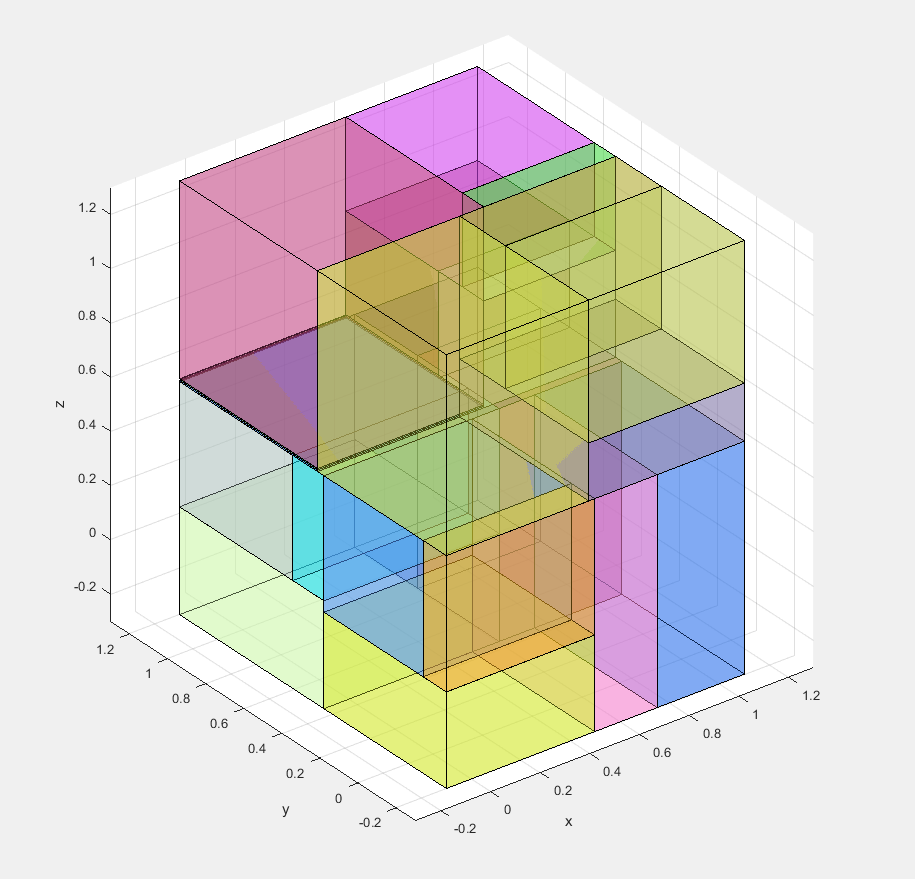
\includegraphics[width=0.9\textwidth]{images/squares.png}
\caption{Example of KD tree partitions}
\end{figure}

\subsubsection{2D animation of tree building}
When prototyping the code in MATLAB, we generated animated visualizations of the construction of a 2D tree. Due to the format, we cannot include the animation within this paper, but it shall be included in the presentation.


\subsubsection{3D tree partitions from different orientations}
Another testing method we performed during our development was validation through variation of input parameters. We held constant the number of data points read, the searching point and search radius, but varied the number of nodes that were used in the process. Then we had each node output the number of data points within their tree that fell within the search point and radius. Although the number of points per tree would vary depending upon the number of nodes used, the sum of all those points would remain constant. From this test we confirmed that the search tree was working as intended. 

\subsection{Other}
During the testing process we also varied the searching parameter radius in two ways. First, we made the search radius very large and as expected we encapsulated all points. Second, we reduced the search radius and the search point so that it should only include a single location and our results were perfect. 

%%%%%%%%%
%
% Section: Results
%
%%%%%%%%%

\section{Results}

% JJ


% JJ

%%%%%%%%%
%
% Subsection: Timing Testing
%
%%%%%%%%%

\subsection{Timing Testing}


\begin{tabular}{r r r r r}
 & \multicolumn{4}{c}{\textbf{Execution times (seconds)}} \\
\textbf{Total Lines} & \underline{32 Cores} & \underline{64 Cores} & \underline{128 Cores} & \underline{200 Cores} \\
       50,000 &   0.55 &     0.57 &     15.49 & 15.45 \\
      500,000 &   4.18 &     5.51 &      4.06 & 9.18 \\
   5,000,0000 &  39.49 &    50.01 &           & 65.05 \\
   50,000,000 & 234.73 &   404.49 &           & 574.71 \\
  500,000,000 &        & 2,094.11 &  3,685.35 & \\
1,000,000,000 &        & 4,146.69 &           &  \\
2,000,000,000 &        &          &           & 21,355.30 \\ 
\end{tabular}

\begin{figure}
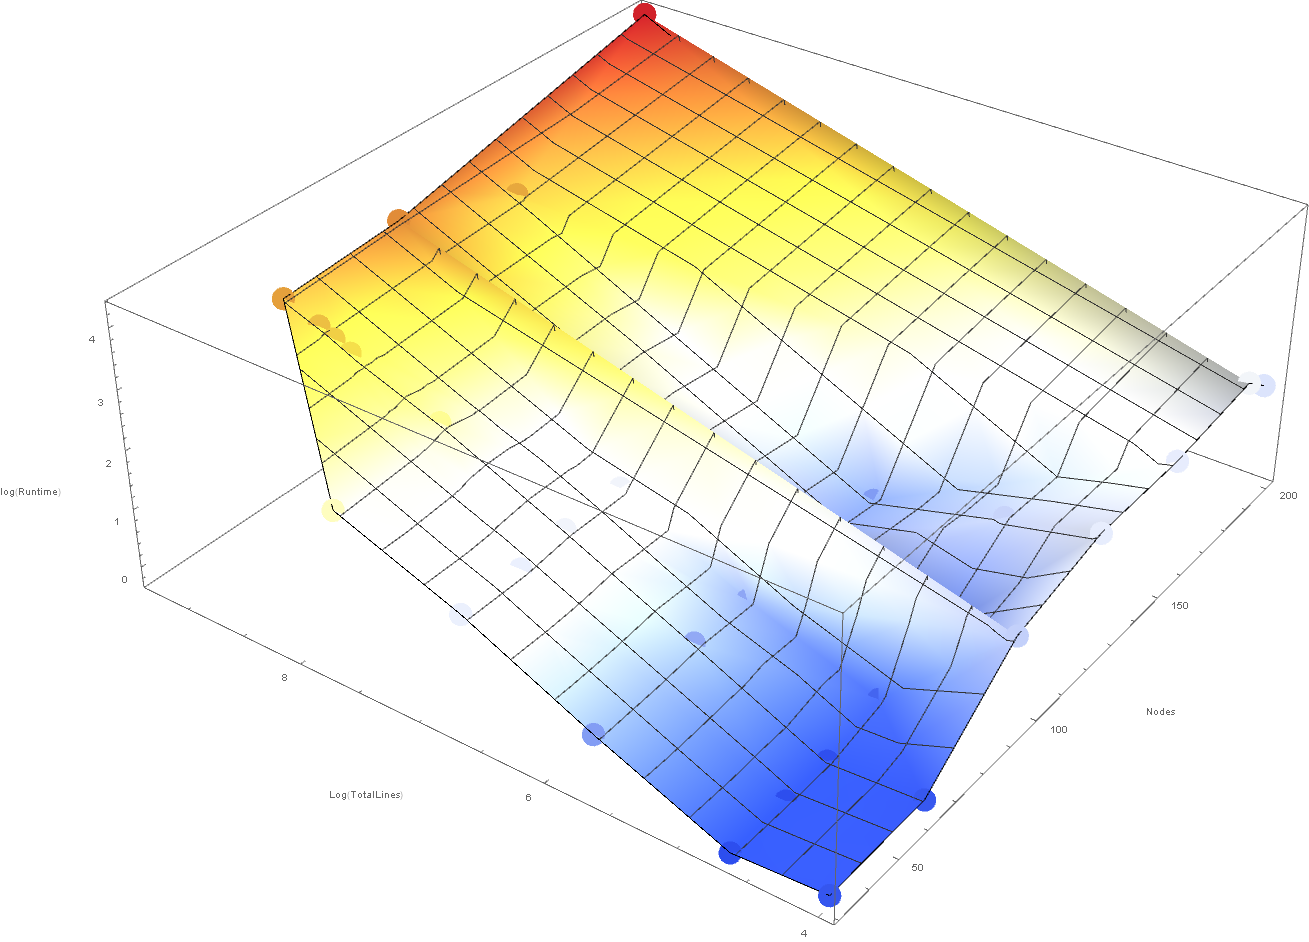
\includegraphics[width=0.9\textwidth]{./images/runtimes.png}
\caption{Execution time versus nodes and total lines}
\end{figure}


\begin{figure}
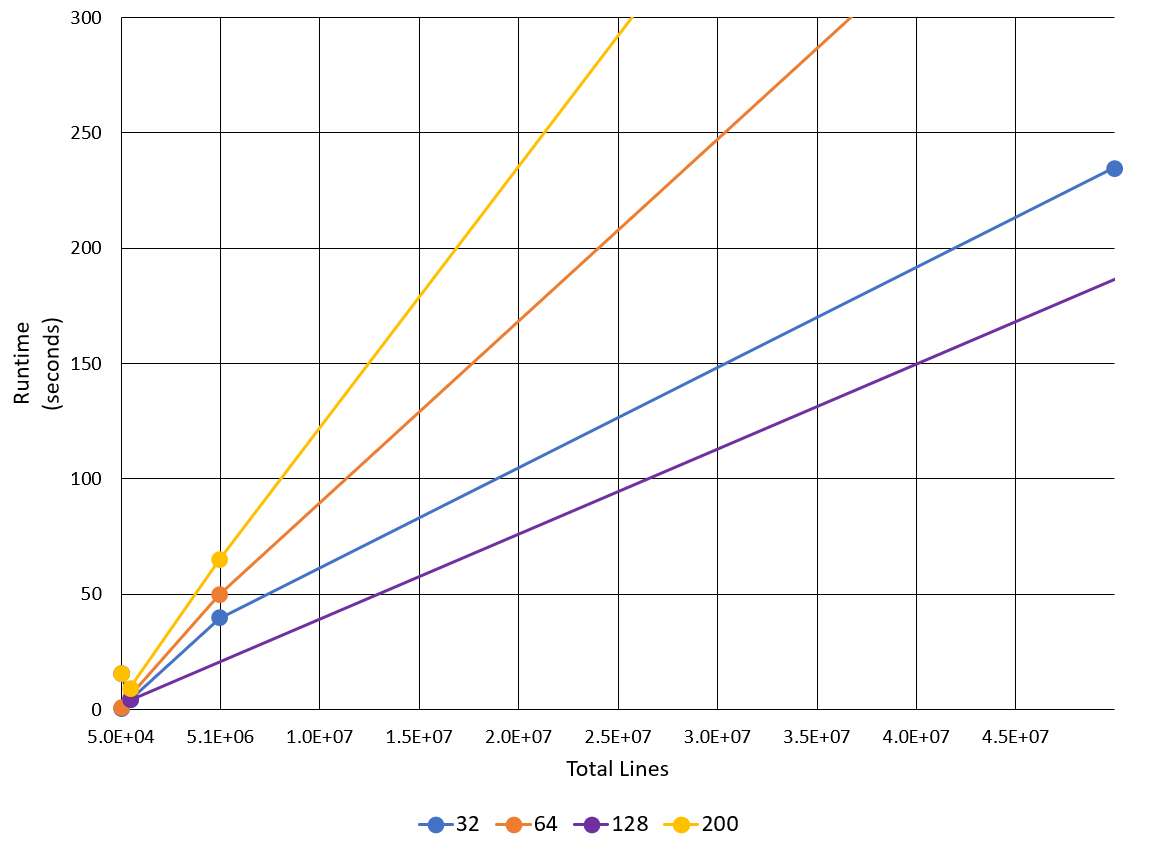
\includegraphics[width=0.9\textwidth]{./images/Runtime1.png}
\caption{Execution time versus nodes for total lines from 50,000 to 50,000,000}
\end{figure}


\begin{figure}
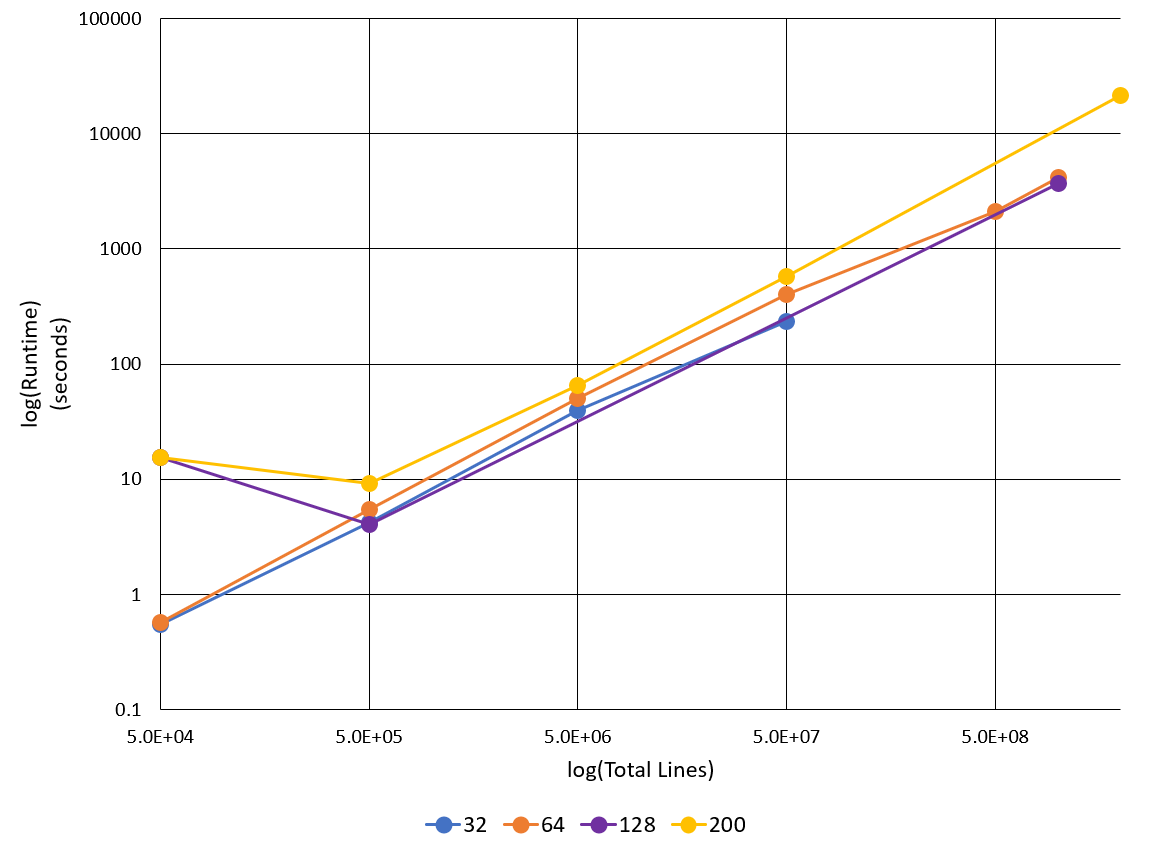
\includegraphics[width=0.9\textwidth]{./images/Runtime2.png}
\caption{Execution time versus nodes and total lines}
\end{figure}

\begin{figure}
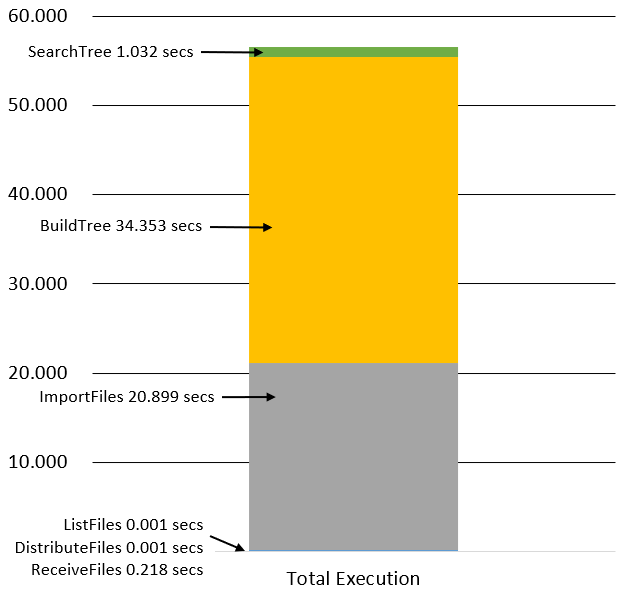
\includegraphics[width=0.9\textwidth]{./images/Runtime3.png}
\caption{Execution time by function for 5,000,000 total lines and 1,000 search rows}
\end{figure}


%%%%%%%%%
%
% Subsection: Search Results
%
%%%%%%%%%

\subsection{Search Results}

The program exports a table at the end of the run displaying the number of points contained in each of three radii centered at each row of points from  \texttt{datafile00501.txt}. The first twenty rows of the output are shown below:

\begin{verbatim}
POINTS FOUND:
 X             Y             Z                   0.01          0.05          0.10
------------  ------------  ------------  ------------  ------------  ------------
    0.581959      0.721012      0.969341        917205      55498018      92120227
    0.894312      0.362959      0.447526         13375       1634169      12135389
    0.801765     -0.037433      0.616920          4026        490535       3837163
    0.685972      0.346683      0.388596         29251       3420777      22785611
    0.716828      0.953059      0.275552          3771        462728       3675457
    0.113410      0.650905      0.795308        797814      53199022      78642100
    0.125404      0.282296      0.536048          1473        187628       1556214
    0.557424      0.471667     -0.075745          1559        190467       1523646
    0.557737      0.697675      0.934643        819217      52896281      92109359
    0.353073      0.840097     -0.000039          1631        195440       1564030
    0.365097      0.064303      0.803032         13811       1693414      12855261
    0.917744      0.511031      1.053122        180759      18109472      67214583
    0.611690     -0.057995      0.263766          1519        186829       1523365
    0.302634      0.128243      0.582824         13350       1586273      11476583
    0.081476     -0.081441      0.254356       2146813      64790807      70678329
    0.215516      0.171119      0.695714          5494        713031       5878422
    0.783198      0.920994      0.874636          2626        317146       2514096
    1.057458      0.734861      0.620092          2985        357166       2338251
    0.399678     -0.069887      0.666980         12781       1560145      11866273
    0.823353      0.852015     -0.053596          3058        371959       2943893
\end{verbatim}

The program was tested using 



%%%%%%%%%%%%%
%%%
%%% Conclusions
%%%
%%%%%%%%%%%%%

\section{Conclusions}
% everyone
This project was an excellent test for managing MPI in the context of large amounts of data and long run times. It also provided an opportunity to work as a well-functioning team and develop a synergistic group dynamic. We were able to overcome significant setbacks. Below is a summary of different aspects of our performance, including some challenges which we struggled with as well as our successes and possible future work.

\begin{mdframed}[backgroundcolor=red!20]
	Challenges:
	\begin{itemize}
		\item \texttt{parallelSort} conversions
		\item memory leaks
		\item \texttt{malloc} when you should \texttt{realloc}
		\item multiple communicators (comm)
		\item \texttt{adaptBins} convergence problems
		\item debug print statement clutter
		\item array out of bounds issues
		\item inconsistent usage pointer-to-pointer calls for *data[] and *rows (due to \texttt{swapArrayParts})
		\item no planning for function arguments and return values (constant editing of h-files)
		\item testing was difficult due to cluster overloading and hardware errors
	\end{itemize}
\end{mdframed}

\begin{mdframed}[backgroundcolor=green!20]
	Successes:
	\begin{itemize}
		\item few merge conflicts and fast debugging through extreme coding and Git branches
		\item visualizing output through MATLAB
		\item efficient delegation of tasks
	\end{itemize}
\end{mdframed}

\begin{mdframed}[backgroundcolor=blue!20]
	Future work:
	\begin{itemize}
		\item cloud computing
		\item use of coding techniques for personal research
	\end{itemize}
\end{mdframed}

%%%%%%%%%%%%%%%
%
% Recommendations
%
%%%%%%%%%%%%%%%

\subsection{Recommendations}

The following recommendations could improve the course when offered next:

\begin{itemize}
    \item Assign a job queue to each team with dedicated nodes for each to eliminate resource conflicts between teams.
    \item 
\end{itemize}


%%%%%%%%%%%%%%%
%
% Links
%
%%%%%%%%%%%%%%%

\subsection{Links}

\begin{verbatim}
* k-d tree repo
  https://github.com/jjlay/COMS7900kdTree

* Production source
  https://github.com/jjlay/COMS7900kdTree/tree/master/code/kdTree/parallelApproved

* Paper
  https://github.com/jjlay/COMS7900kdTree/tree/master/paper

* Presentation
  https://github.com/jjlay/COMS7900kdTree/tree/master/presentation
  
* ParallelSort
  https://github.com/jjlay/COMS7900kdTree/tree/master/code/parallelSort
\end{verbatim}


%%%%%%%%%%%%%
%%% NEW SECTION %%%
%%%%%%%%%%%%%
% \section{Bibliography}

\end{document}
